% =========================================================================
%  WG-Fusion -- CVPR-style manuscript
%  All numbers generated from experiment artifacts (see paper/make_figures.py
%  and ../../PROGRESS_REPORT.md). Figures live in paper/figures/.
% =========================================================================
\documentclass[10pt,twocolumn,letterpaper]{article}

\usepackage[review]{cvpr}
\usepackage{graphicx}
\usepackage{amsmath}
\usepackage{amssymb}
\usepackage{booktabs}
\usepackage{multirow}
\usepackage{xcolor}
\usepackage{tikz}
\usetikzlibrary{arrows.meta}
\usepackage{caption}
\usepackage{subcaption}

\definecolor{cvprblue}{rgb}{0.21,0.49,0.74}
\usepackage[breaklinks,colorlinks,allcolors=cvprblue]{hyperref}

\newcommand{\TODO}[1]{{\color{red}\textbf{[TODO: #1]}}}

\def\confName{CVPR}
\def\confYear{2027}

\title{WG-Fusion: Window-Graph Cross-Modal Fusion for\\Paired Infrared--Visible Object Detection}

\author{Anonymous submission}

\begin{document}
\maketitle

% ===================================================================== abstract
\begin{abstract}
Infrared (IR) and visible (RGB) cameras are increasingly co-mounted on aerial
platforms, so paired IR--RGB object detection---not single-modality
detection---is the realistic deployment setting. Yet many fusion designs are
evaluated against weak or unmatched baselines, leaving open whether a
structured cross-modal interaction is actually needed at a fixed training
budget. We introduce \textbf{WG-Fusion}, a dual-stream detector in which each
of the three backbone levels is fused by a single window-graph attention layer:
every IR feature-map cell is a node that aggregates from its eight grid
neighbours and from a $3\times3$ cross-modal window of RGB cells, with edge
features (offset, cosine similarity, node quality) and an IR-anchored gated
residual. Trained on DroneVehicle with the reference recipe at matched budget,
WG-Fusion raises the locked 8,980-image test AP from $0.5783$ (IR-only) to
$\mathbf{0.5988}$ ($+2.08$~pp, paired bootstrap 95\% CI $[+1.71,+2.42]$) and
significantly beats a concat fusion baseline ($+0.59$~pp, CI $[+0.25,+0.89]$).
On the 1,469-image split used by prior work it reaches $85.8$/$64.8$ mAP$_{50}$
/ mAP$_{50{:}95}$, competitive with recent attention and Mamba fusion methods.
Ablations show that two stacked graph hops, a wider graph ($d{=}192$) and
semantic-kNN edges do not improve the mean, while a warm-started fine-tune
degrades it: under a matched recipe the \emph{formulation}---mid-level,
IR-anchored, local cross-modal exchange---drives the gain, not graph
hyper-parameters. We release code, locked test protocols and every training
curve.
\end{abstract}

% ===================================================================== intro
\section{Introduction}

Object detection from unmanned aerial vehicles (UAVs) must work across the full
diurnal cycle. A visible (RGB) camera provides texture, colour and fine
boundaries but degrades at night, in glare, fog and motion blur; a thermal
infrared (IR) camera sees vehicles as heat sources independent of illumination
but lacks texture and can merge adjacent objects. The two sensors are
complementary, and modern drone payloads carry both---usually already
geo-aligned.

This makes \emph{paired} IR--RGB detection the natural formulation, and it has
motivated three families of methods: early (input-level) fusion, late
(box-level) fusion, and mid-level feature fusion. Early fusion is sensitive to
photometric differences between the modalities; late fusion cannot exploit
cross-modal evidence during feature learning. Mid-level fusion is the
strongest design point, and increasingly structured: cross-attention
(ICAFusion~\cite{icafusion}, PNAFusion~\cite{pnafusion}), state-space
interaction (AMSRDet~\cite{amsrdet}, COMO~\cite{como}), or graph/hypergraph
reasoning (HyperDet~\cite{hyperdet}).

Two questions remain under-addressed in that literature. First, \emph{is a
structured module necessary at a fixed budget?} Many fusion papers compare
against single-modality detectors with different backbones, resolutions or
training schedules, so the reported gain mixes architecture with recipe.
Second, \emph{which part of a graph formulation actually matters?} Graph
methods introduce nodes, edge sets, edge features and depth, and ablations
usually vary them one at a time on the validation split that is also used for
selection.

We address both on DroneVehicle~\cite{dronevehicle}, the largest paired
aerial IR--RGB detection benchmark, with a deliberately controlled
methodology: one detector (dual-stream YOLO12s~\cite{yolo12}), one recipe, one
seed, and two evaluation axes---the 1,469-image split on which prior work
reports (comparable to the literature) and a locked 8,980-image test set never
used for selection (the rigorous claim).

Our contributions are:
\begin{itemize}
  \item \textbf{WG-Fusion}, a window-graph attention layer applied at P3/P4/P5
        of a dual-stream YOLO12s: IR nodes, eight grid edges plus a $3\times3$
        cross-modal window, five edge features, masked softmax and an
        IR-anchored gated residual. The layer is a near-identity correction at
        initialisation.
  \item \textbf{A controlled evaluation} on DroneVehicle with matched recipe
        and budget: mid-level fusion improves locked-test AP by
        $+1.5$--$+2.1$~pp over IR-only across five fused variants, and the
        window graph significantly beats concat fusion by $+0.59$~pp
        (CI excludes zero).
  \item \textbf{A negative-result ablation suite}: depth (two hops), width
        ($d{=}192$), semantic-kNN edges and warm-started fine-tuning are
        neutral or harmful. The graph's \emph{form} matters more than its
        hyper-parameters.
  \item A \textbf{headroom analysis} showing that fusion captures most of the
        overall labelled-oracle gain, with the largest remaining headroom on
        small objects ($+6.7$~pp recall).
\end{itemize}

% ===================================================================== related
\section{Related Work}
\paragraph{IR-only and RGB-only detection.}
Single-modality detectors dominate deployment: YOLO-family models~\cite{yolo12}
are the usual aerial workhorses, and DroneVehicle's original baselines
report IR and RGB detectors separately~\cite{dronevehicle}. With paired data,
the natural reference is the IR-only detector, because thermal imagery is the
more robust modality at night.

\paragraph{Early and late fusion.}
Early fusion stacks the modalities into a six-channel input; it is cheap but
cannot model modality-specific statistics. Late fusion combines detections or
boxes, e.g. weighted box fusion (WBF)~\cite{wbf}; it is training-free but
cannot improve features. Both are included here as references.

\paragraph{Mid-level fusion.}
CFT~\cite{cft} introduced cross-modal transformers over two-stream features;
ICAFusion~\cite{icafusion} adds iterative bidirectional cross-attention;
PNAFusion~\cite{pnafusion} restricts cross-attention to local deformable
neighbourhoods, which also cuts compute. Mamba/SSM designs
(AMSRDet~\cite{amsrdet}, COMO~\cite{como}, MambaRefine~\cite{mambarefine})
exchange cross-modal information through linear-complexity state-space blocks.
IV-PAFNet~\cite{ivpafnet} combines IR purification with visible-guided
alignment on an RT-DETR backbone.

\paragraph{Graph and hypergraph fusion.}
HyperDet~\cite{hyperdet} builds dynamic hyperedges over semantically consistent
instances and is the current DroneVehicle frontier. Our window graph differs
in being \emph{local} (bounded neighbourhood), \emph{fixed-geometry} (no
instance construction) and \emph{residual on the IR stream}, which keeps it
cheap and stable at initialisation.

\paragraph{Benchmarks and protocol.}
DroneVehicle~\cite{dronevehicle} provides 28{,}439 aligned IR--RGB pairs with
oriented vehicle boxes. The official split is 17{,}990 train / 1{,}469
validation / 8{,}980 test. Most published numbers are reported on the
1,469-image split---sometimes called ``test'' in those papers---and are
obtained after selecting the best checkpoint on that same split. We therefore
report that split for comparability, and a pre-registered locked split for our
own claims (\S\ref{sec:protocol}).

% ===================================================================== protocol
\section{Problem Statement, Data and Protocol}\label{sec:protocol}

\paragraph{Task.}
Given an aligned pair $(I_{\mathrm{ir}}, I_{\mathrm{rgb}})$, predict boxes and
labels for five vehicle classes. The detector is trained on paired data and
evaluated with COCO-style AP (mAP$_{50{:}95}$, AP$_{50}$, AP$_{\mathrm{s}}$,
AP$_{\mathrm{m}}$, AP$_{\mathrm{l}}$) using pycocotools.

\paragraph{Data.}
DroneVehicle, official split: 17{,}962 training pairs usable after removing 28
frames with missing annotations, 1{,}469 validation pairs, 8{,}980 test pairs.
Training supervision uses thermal labels for the IR stream and visible labels
for the RGB stream; evaluation uses thermal ground truth. The validation split
contains 24{,}490 instances (car 20{,}588; truck 1{,}470; bus 789; van 725;
freight 918), of which 10{,}850 are day and 13{,}640 night frames; by object
size, 3{,}996 are small, 19{,}788 medium and 706 large (Fig.~\ref{fig:dataset}).

\begin{figure}[t]
\centering
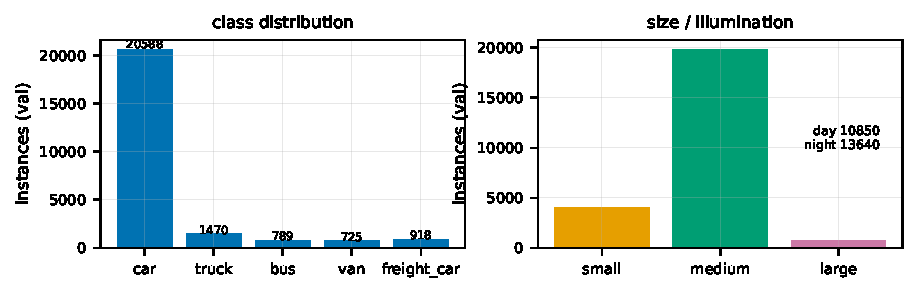
\includegraphics[width=\linewidth]{figures/fig_dataset.pdf}
\caption{DroneVehicle validation split: class distribution (left) and object-size
/ illumination composition (right). Small objects dominate the fusion headroom.}
\label{fig:dataset}
\end{figure}

\paragraph{Why DroneVehicle.}
It is the largest paired aerial IR--RGB detection benchmark with a standard
split, dense small vehicles, and both day and night coverage---exactly the
conditions where fusion should matter. Multi-dataset validation (FLIR, VEDAI,
M3FD) is left to future work.

\paragraph{The two evaluation axes.}
\emph{Val axis.} The 1{,}469-image split is used for checkpoint selection (as
in prior work) and is the axis on which published DroneVehicle numbers are
reported; we compare there with a caveat that selection and reporting coincide.
\emph{Locked test axis.} The 8{,}980-image split is never used for selection:
checkpoints are fixed by validation, then predictions are exported once, and
the protocol (checkpoint hash, recipe hash, metric) is recorded in a lock file
before any test prediction exists. Seed-0 results are single-seed; a second
seed of the main arm is reported where available.

\paragraph{Oracle headroom.}
To bound what fusion can achieve, we compute a per-annotation oracle: an
annotation counts as detected if either the IR-only or the RGB-only detector
recall set contains it. On validation, the IR-only detector recalls 91.79\%,
the RGB-only 79.81\%, and the oracle 94.97\% ($+3.18$~pp). The gap is
$+2.25$~pp at night, $+4.34$~pp by day, and $+6.73$~pp for small objects
(Fig.~\ref{fig:oracle})---the largest structured headroom.

% ===================================================================== method
\section{Method: WG-Fusion}\label{sec:method}

\subsection{Overview}
WG-Fusion is a dual-stream detector. Both streams are YOLO12s
backbones~\cite{yolo12}; the IR stream is initialised from COCO weights with
per-filter channel-mean grayscale adaptation of the stem, and the RGB stream
keeps the original filters. At each of the three backbone output levels
(P3: $80\times64$, P4: $40\times32$, P5: $20\times16$ for $640\times512$
inputs) a window-graph attention layer fuses the two feature maps and returns a
map of the same shape, which replaces the level's anchor in the stock PAN neck
and detection head (Fig.~\ref{fig:arch}). Boxes and labels therefore come from
the unmodified detector; fusion only rewrites the three anchor maps.

\subsection{Graph construction}
\paragraph{Nodes.} Nodes are the $N=H\cdot W$ cells of the IR feature map.
Each node carries a $d$-dimensional projection of its IR feature
($h_i=\mathrm{proj}_{\mathrm{ir}}(f_{\mathrm{ir}})$); RGB cells are twin nodes
with global ids $N,\dots,2N-1$ and a separate projection. Only IR nodes are
updated; RGB nodes act as sources.

\paragraph{Edges.} Every IR node receives messages from $K=8+(2r+1)^2$
neighbours at radius $r=1$: its eight grid neighbours inside the IR map, and
the nine RGB nodes in the $3\times3$ window centred on the same location
(the co-located RGB node included). The tables are fixed, precomputed per
$(H,W)$ and cached; boundary cells use a validity mask, and softmax is
restricted to valid neighbours.

\paragraph{Edge features.} Each edge carries
$e_{ij}=[\Delta x/\rho,\ \Delta y/\rho,\ \cos(W h_i, W h_j),\ q_i,\ q_j]$,
with $\rho=\max(r,1)$, and node qualities
$q_\ast=\sigma(\mathrm{Conv}_{1\times1}(f_\ast))$ in $(0,1)$ produced by a
head shared between modalities. Positions, content similarity and per-node
reliability therefore all enter the attention.

\subsection{Window-graph attention}
With $\mathcal{N}(i)$ the valid neighbours of node $i$:
\begin{align}
\ell_{ij} &= \mathrm{LeakyReLU}\!\left(a^{\top}[Wh_i\,\|\,Wh_j\,\|\,W_e e_{ij}]\right),\\
\alpha_{ij} &= \mathrm{softmax}_{j\in\mathcal{N}(i)}(\ell_{ij}),\\
\mathrm{agg}_i &= \sum_{j\in\mathcal{N}(i)} \alpha_{ij}\, W_v h_j,\\
g_i &= \sigma\!\left(\mathrm{MLP}([h_i\,\|\,\mathrm{agg}_i])\right),\\
h_i' &= h_i + g_i\odot \mathrm{agg}_i,\qquad
\Delta = \mathrm{out}(h'),\qquad f_{\text{fused}} = f_{\mathrm{ir}} + \Delta .
\end{align}
The gate MLP's final bias is $-4.0$ and the output projection is
small-initialised, so at step zero the module is a near-identity correction on
the IR stream: a fused model never starts worse than its IR-only reference.
Attention is computed in fp32 even under AMP, and non-finite values raise
rather than propagate. One layer adds
$P=3Cd+5d^2+6d+E^2+2E+2C+1$ parameters per level with $E=5$ (0.64M for the
three levels at $d{=}128$).

\begin{figure*}[t]
\centering
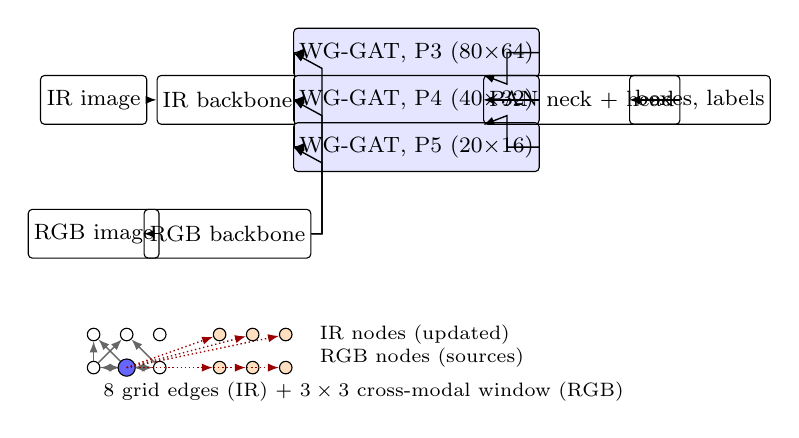
\begin{tikzpicture}[
  font=\footnotesize,
  box/.style={draw,rounded corners=1.5pt,minimum height=0.62cm,minimum width=1.35cm,align=center,inner sep=2pt},
  fuse/.style={draw,fill=blue!10,rounded corners=1.5pt,minimum height=0.62cm,minimum width=1.9cm,align=center,inner sep=2pt},
  arr/.style={-{Latex[length=1.4mm]},line width=0.5pt}]
  % streams
  \node[box] (ir)  at (0.0,1.9) {IR image};
  \node[box] (ibb) at (1.7,1.9) {IR backbone};
  \node[box] (rgb) at (0.0,0.2) {RGB image};
  \node[box] (rbb) at (1.7,0.2) {RGB backbone};
  % fuse blocks
  \node[fuse] (f3) at (4.1,2.5) {WG-GAT, P3 ($80{\times}64$)};
  \node[fuse] (f4) at (4.1,1.9) {WG-GAT, P4 ($40{\times}32$)};
  \node[fuse] (f5) at (4.1,1.3) {WG-GAT, P5 ($20{\times}16$)};
  % neck + head
  \node[box,minimum width=1.5cm] (neck) at (6.2,1.9) {PAN neck + head};
  \node[box,minimum width=1.1cm] (out)  at (7.7,1.9) {boxes, labels};
  % arrows
  \draw[arr] (ir) -- (ibb);
  \draw[arr] (rgb) -- (rbb);
  \draw[arr] (ibb.east) -- (2.55,1.9) -- (2.55,2.5) -- (f3.west);
  \draw[arr] (ibb.east) -- (f4.west);
  \draw[arr] (ibb.east) -- (2.55,1.9) -- (2.55,1.3) -- (f5.west);
  \draw[arr] (rbb.east) -- (2.9,0.2) -- (2.9,2.3) -- (f3.west);
  \draw[arr] (rbb.east) -- (2.9,0.2) -- (2.9,1.7) -- (f4.west);
  \draw[arr] (rbb.east) -- (2.9,0.2) -- (2.9,1.1) -- (f5.west);
  \draw[arr] (f3.east) -- (5.25,2.5) -- (5.25,2.1) -- (neck.north west);
  \draw[arr] (f4.east) -- (neck.west);
  \draw[arr] (f5.east) -- (5.25,1.3) -- (5.25,1.7) -- (neck.south west);
  \draw[arr] (neck) -- (out);
  % graph inset
  \begin{scope}[shift={(0.0,-1.5)}]
    \foreach \x in {0,1,2} \foreach \y in {0,1} {
      \node[draw,circle,inner sep=1.6pt,fill=white] (a\x\y) at (\x*0.42,\y*0.42) {};
      \node[draw,circle,inner sep=1.6pt,fill=orange!25] (b\x\y) at (1.6+\x*0.42,\y*0.42) {};
    }
    \foreach \x/\y/\u/\v in {0/0/1/0,0/0/0/1,0/0/1/1,1/0/2/0,1/0/0/1,1/0/0/0,2/0/1/0,2/0/1/1}
      \draw[arr,black!60] (a\x\y) -- (a\u\v);
    \node[draw,circle,inner sep=2.2pt,fill=blue!60] at (0.42,0.0) {};
    \foreach \x in {0,1,2} \foreach \y in {0,1}
      \draw[arr,red!60!black,densely dotted] (0.42,0.0) -- (b\x\y);
    \node[font=\scriptsize,anchor=west] at (2.75,0.42) {IR nodes (updated)};
    \node[font=\scriptsize,anchor=west] at (2.75,0.12) {RGB nodes (sources)};
    \node[font=\scriptsize,anchor=west] at (0.0,-0.30) {8 grid edges (IR) + $3\times3$ cross-modal window (RGB)};
  \end{scope}
\end{tikzpicture}
\caption{WG-Fusion. A dual-stream YOLO12s is fused at each backbone level by a
window-graph attention layer; fused P3/P4/P5 replace the anchors of the stock
neck and head. \emph{Inset}: every IR node receives eight grid edges from the
IR map and a $3\times3$ window of RGB nodes; edge features are
$(\Delta x,\Delta y,\cos,q_i,q_j)$ and the update is an IR-anchored gated
residual.}
\label{fig:arch}
\end{figure*}

\subsection{Training}
The model is trained end-to-end with the stock YOLO detection loss (CIoU box,
BCE class, DFL) through the head, neck, both backbones and all fusion layers.
The recipe matches the IR-only reference exactly: SGD-style optimizer, initial
LR $0.01$, final LR fraction $0.01$ over 100 epochs, momentum $0.937$, batch
16 with gradient accumulation to a nominal batch of 64, mosaic closing at
epoch 90, patience 30, seed 0. No test data is used at any point.

% ===================================================================== results
\section{Experiments}

\subsection{Setup}
All arms use the same detector, data, augmentation, schedule and seed; the only
difference is the fusion module (or its absence). Training runs on a single
48~GB GPU; fusion layers run in fp32 under AMP. AP is computed with
pycocotools; confidence intervals come from paired image-level bootstrap with
500 resamples, resampling the same images for every model.

\subsection{Main results: locked test}
Table~\ref{tab:test} reports the locked 8,980-image test set. Every fused arm
beats the IR-only reference with CIs excluding zero. WG-Fusion (E30) is the
best single model at 0.5988 AP, and the paired bootstrap against the concat
baseline is significant ($+0.59$~pp, CI $[+0.25,+0.89]$). The two-hop variant
(E41) is statistically indistinguishable from WG-Fusion ($-0.25$~pp,
CI $[-0.59,+0.04]$) but has the best small-object AP (0.2388); the wider
graph ($d{=}192$) is significantly worse ($-0.75$~pp).

\begin{table}[t]
\centering
\small
\setlength{\tabcolsep}{4pt}
\begin{tabular}{@{}lcccccc@{}}
\toprule
Method & AP & AP$_{50}$ & AP$_{\mathrm{s}}$ & AP$_{\mathrm{m}}$ & AP$_{\mathrm{l}}$ & $\Delta$ vs IR \\
\midrule
IR-only (E00)      & 0.5783 & 0.7628 & 0.1866 & 0.5750 & 0.6298 & -- \\
Concat (E10)       & 0.5931 & 0.7754 & 0.2381 & 0.5912 & 0.5904 & $+1.49$ \\
\textbf{WG-Fusion (E30)} & \textbf{0.5988} & \textbf{0.7819} & 0.2336 & \textbf{0.5951} & 0.6245 & $\mathbf{+2.08}$ \\
\quad 2 hops (E41) & 0.5969 & 0.7784 & \textbf{0.2388} & 0.5939 & 0.6181 & $+1.83$ \\
\quad semantic edges (E35) & 0.5943 & 0.7770 & 0.2273 & 0.5921 & 0.6217 & $+1.60$ \\
\quad $d{=}192$    & 0.5914 & 0.7760 & 0.2364 & 0.5881 & 0.6231 & $+1.33$ \\
\bottomrule
\end{tabular}
\caption{Locked 8,980-image test set (thermal GT, single seed). $\Delta$ vs IR
gives the paired-bootstrap mean; all CIs exclude zero (see
Fig.~\ref{fig:testap}). WG-Fusion is the best single model; the two-hop variant
trades overall AP for the best small-object AP.}
\label{tab:test}
\end{table}

\begin{figure}[t]
\centering
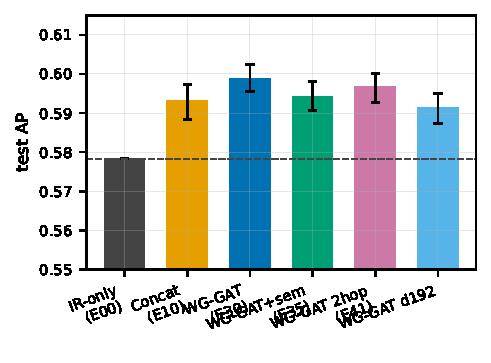
\includegraphics[width=\linewidth]{figures/fig_test_ap.pdf}
\caption{Locked-test AP with paired-bootstrap 95\% CIs (dashed line: IR-only).
All fused arms are above the IR reference; WG-Fusion leads.}
\label{fig:testap}
\end{figure}

\begin{figure}[t]
\centering
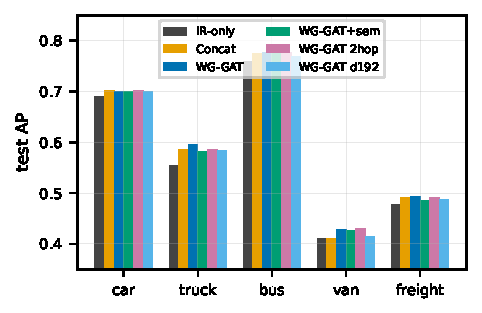
\includegraphics[width=\linewidth]{figures/fig_per_class.pdf}
\caption{Per-class test AP. WG-Fusion leads on truck, van and freight; concat
leads slightly on car and bus.}
\label{fig:perclass}
\end{figure}

\begin{figure}[t]
\centering
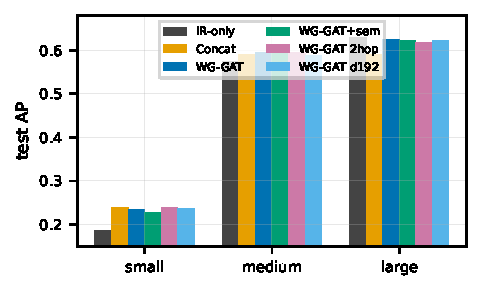
\includegraphics[width=\linewidth]{figures/fig_scale.pdf}
\caption{Scale breakdown. Concat buys the largest small-object gain but loses
large-object AP (0.590 vs 0.630 for IR-only); the graph arms keep large-object
performance almost intact while gaining nearly as much on small objects.}
\label{fig:scale}
\end{figure}

\subsection{Comparison with published results}
Table~\ref{tab:sota} places WG-Fusion on the 1,469-image split used by prior
work. We report the comparison as \emph{context}, not as a controlled ranking:
the same method can differ by up to 9~pp between tables (e.g.\ ICAFusion
appears as 75.4, 78.6 and 84.8 in different sources), because split, box
protocol (oriented vs horizontal), label stream and reproduction all vary. On
this axis WG-Fusion (85.8/64.8) is above every 2023--2025 entry, including
C2DFF-Net (85.7/65.2), and 0.5--1.7~pp behind the February-2026 hypergraph
frontier (HyperDet). Notably, the IR-only baseline alone (84.2/63.1) already
matches or beats most published \emph{fused} methods through 2024, which is why
we treat the controlled $\Delta$ over IR-only as the meaningful number.

\begin{table}[t]
\centering
\small
\setlength{\tabcolsep}{4pt}
\begin{tabular}{@{}llcc@{}}
\toprule
Method & Venue (date) & mAP$_{50}$ & mAP$_{50{:}95}$ \\
\midrule
CFT~\cite{cft} & arXiv'21/TGRS'22 & 84.3 & 61.9 \\
SuperYOLO~\cite{superyolo} & TGRS'23 & 81.4 & 58.6 \\
ICAFusion~\cite{icafusion} (re-run) & PR'24 & 75.4 & 52.6 \\
MGMF~\cite{mgmf} & TGRS'24 & 80.3 & 55.2 \\
C2DFF-Net~\cite{c2dff} & TGRS'25 & 85.7 & 65.2 \\
COMO~\cite{como} & Inf.\ Fusion'26 & 85.3 & 63.4 \\
HyperDet-N~\cite{hyperdet} & JKSU-CIS'26 & 86.4 & 65.9 \\
HyperDet-S~\cite{hyperdet} & JKSU-CIS'26 & 87.5 & 67.1 \\
\midrule
IR-only (ours) & -- & 84.2 & 63.1 \\
\textbf{WG-Fusion (ours)} & -- & \textbf{85.8} & \textbf{64.8} \\
\bottomrule
\end{tabular}
\caption{Context on the 1,469-image DroneVehicle split used by prior work
(values as reported by HyperDet's single-protocol table, which re-runs all
methods). Not a controlled comparison; see text.}
\label{tab:sota}
\end{table}

\subsection{Ablations}
Table~\ref{tab:abl} varies one factor at a time under the same recipe.
\emph{Depth}: a second graph hop (E41) is neutral overall but improves small
objects and the van class. \emph{Width}: $d{=}192$ is significantly worse on
test despite an equal validation score and the highest validation mAP$_{50}$,
illustrating why we select on validation but report on the locked test.
\emph{Edge content}: semantic-kNN edges (E35) are neutral.
\emph{Training technique}: initialising both streams from our converged
IR-only and RGB-only detectors (warm start) and fine-tuning for 50 epochs
peaks at 0.6217 validation, far below from-scratch training---the converged
initialisation leaves no room for the fusion to improve.
\emph{Receptive field}: a $5\times5$ window ($r{=}2$) exceeds batch-16 memory,
so it is not comparable under this budget.

\begin{table}[t]
\centering
\small
\setlength{\tabcolsep}{4pt}
\begin{tabular}{@{}lccc@{}}
\toprule
Variant & val mAP$_{50{:}95}$ & test AP & $\Delta$ test vs WG \\
\midrule
WG-Fusion (1 hop, $d{=}128$) & 0.6484 & \textbf{0.5988} & -- \\
2 hops (E41) & 0.6471 & 0.5969 & $-0.25$ (n.s.) \\
$d{=}192$ & 0.6476 & 0.5914 & $-0.75$ (sig.) \\
semantic-kNN edges (E35) & 0.6471 & 0.5943 & $-0.45$ \\
warm-start fine-tune & 0.6217 & -- & -- \\
$r{=}2$ window & OOM & -- & -- \\
\midrule
IR-only & 0.6306 & 0.5783 & $-2.08$ \\
concat & 0.6538 & 0.5931 & $-0.59$ (sig.) \\
\bottomrule
\end{tabular}
\caption{Ablations. Validation best is at the best epoch; test AP is the locked
one-shot result. Depth and edge content are neutral; capacity hurts; the
warm-started recipe fails.}
\label{tab:abl}
\end{table}

\begin{figure}[t]
\centering
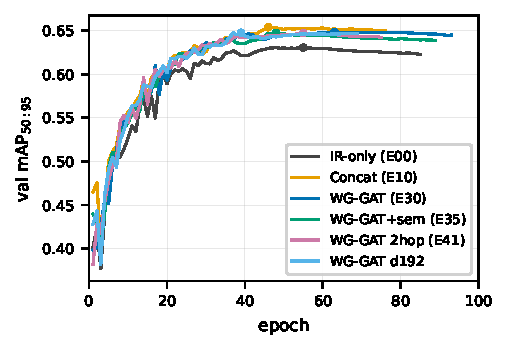
\includegraphics[width=\linewidth]{figures/fig_val_curves.pdf}
\caption{Epoch-matched validation curves. All fused arms track or exceed the
IR-only curve from the first epochs; early stopping is applied per run.}
\label{fig:curves}
\end{figure}

\subsection{Oracle headroom}
Fig.~\ref{fig:oracle} shows the per-annotation oracle. WG-Fusion's $+2.08$~pp
test gain captures a large share of the $+3.18$~pp overall oracle; the largest
remaining structured headroom is on small objects ($+6.73$~pp recall) and at
night ($+2.25$~pp), which motivates future cross-scale edges.

\begin{figure}[t]
\centering
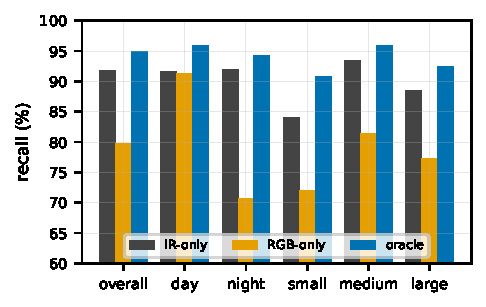
\includegraphics[width=\linewidth]{figures/fig_oracle.pdf}
\caption{Oracle recall by stratum (validation): an annotation is detected if
either single-modality detector recalls it. Small objects carry the largest
headroom.}
\label{fig:oracle}
\end{figure}

\begin{figure}[t]
\centering
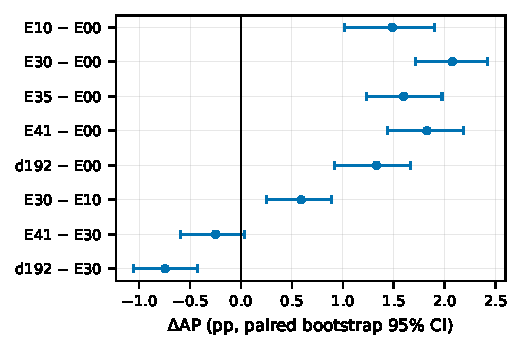
\includegraphics[width=\linewidth]{figures/fig_deltas.pdf}
\caption{Paired-bootstrap $\Delta$AP with 95\% CIs. Against IR-only all fused
arms are positive; WG-Fusion significantly exceeds concat, and capacity
($d{=}192$) is significantly worse than the base graph.}
\label{fig:deltas}
\end{figure}

\subsection{Inference-time ensembles}
Weighted box fusion~\cite{wbf} of the three 100-epoch arms at fixed defaults
(IoU 0.55, one box per source) reaches 0.6211 AP on the locked test, and the
two graph arms alone 0.6128. These are post-hoc, inference-only variants (no
training), reported separately from the trained models; they show that the
arms are complementary, with the concat arm contributing car/bus strength and
the graph arms contributing truck/van/freight.

\subsection{Efficiency}
WG-Fusion adds 0.64M parameters over the dual backbone (15.3M total) and runs
at about 4.9~min/epoch on one 48~GB GPU (21.6~GB peak). The two-hop variant
costs 1.29M fusion parameters, 6.2~min/epoch and 28.2~GB; the $d{=}192$
variant 6.0~min/epoch and 26.5~GB. The semantic-kNN variant is the most
expensive (14.3~min/epoch, 35~GB) because it rebuilds content-dependent edges
every forward.

\subsection{Qualitative analysis}
\TODO{attention-mass heatmaps on grid vs cross-modal edges, $|\Delta|$ maps per
level, day/night detection examples, and confusion matrices (car/van/truck)
will be added here; the fusion modules already expose attention weights, edge
ids and per-node deltas for these plots.}

% ===================================================================== discussion
\section{Discussion and Limitations}
\paragraph{What the results say.}
Under a matched recipe, mid-level fusion reliably improves paired IR--RGB
detection on DroneVehicle ($+1.5$--$+2.1$~pp locked test), and the window graph
is significantly better than plain concat. The graph's structure, however, has
a flat optimum: depth, width and edge content do not move the mean. We read
this as evidence that the \emph{inductive bias}---local cross-modal exchange
applied as an IR-anchored residual---is what matters, and that tuning graph
hyper-parameters is not the path to further gains.

\paragraph{Limitations.}
(i) Single seed for most arms; a second seed of WG-Fusion is reported
separately. (ii) The validation split is also used for selection, as in prior
work; our locked test is the rigorous axis. (iii) The graph is local and
single-scale; cross-scale edges from P4/P5 into P3 are the natural next step
for the small-object headroom. (iv) Only DroneVehicle is covered here;
multi-dataset validation is future work. (v) The two-hop variant's small-object
advantage is not significant overall and needs more seeds to be trusted.

% ===================================================================== conclusion
\section{Conclusion}
We presented WG-Fusion, a window-graph cross-modal fusion layer for paired
IR--RGB detection, and a controlled study on DroneVehicle. WG-Fusion improves
locked-test AP by $+2.08$~pp over the IR-only reference and significantly
beats concat fusion by $+0.59$~pp, while remaining competitive with recent
attention and Mamba methods on the split used by prior work. Ablations show
that graph depth, width and semantic edges are neutral or harmful under a
matched recipe: the formulation, not its hyper-parameters, carries the gain.
We release the code, the pre-registered locks, and every training curve.

{\small
\bibliographystyle{ieeenat_fullname}
\bibliography{main}
}

\end{document}
